\section{Method}\label{pca:method}

\begin{figure}
\centering
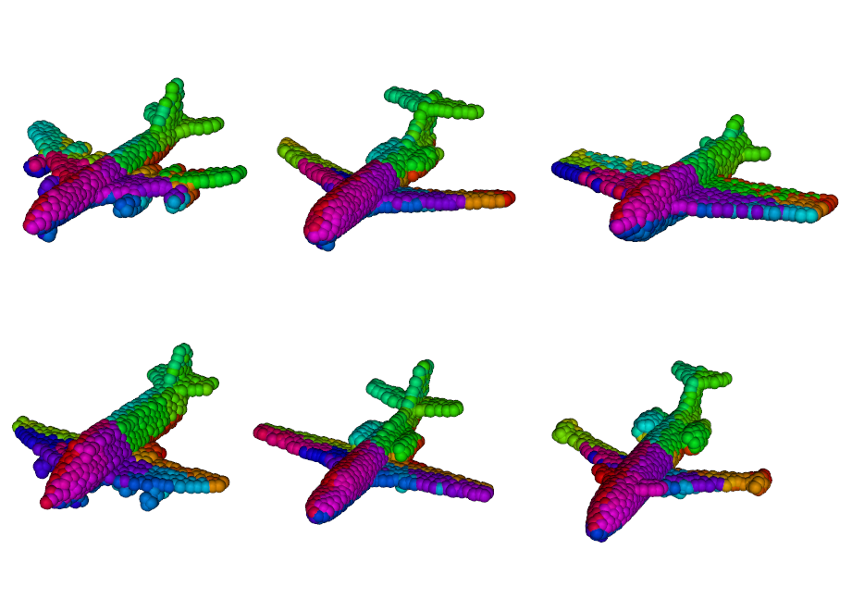
\includegraphics[width=0.49\linewidth]{PCAGAN/images/airplanes_sorting_new2.png}

\includegraphics[height=1.4in]{PCAGAN/images/vline.png}
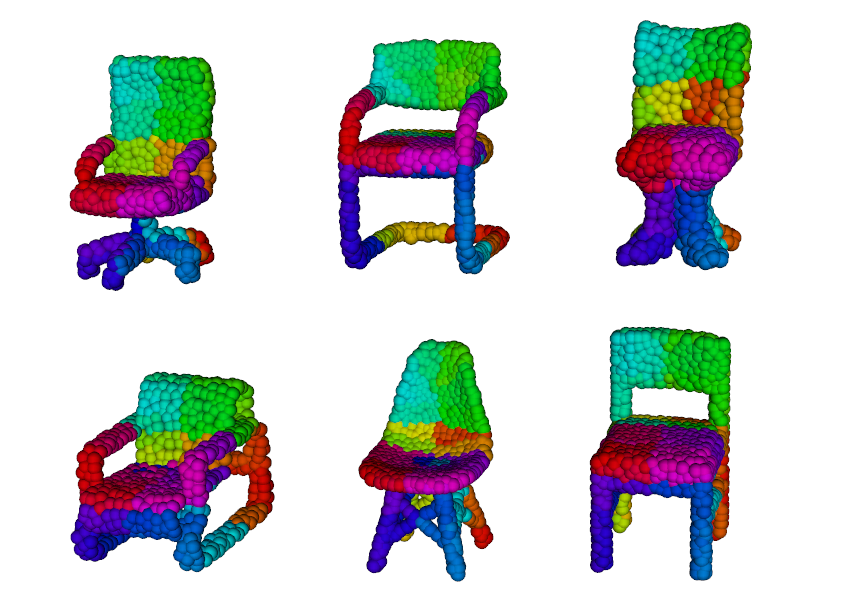
\includegraphics[width=0.49\linewidth]{PCAGAN/images/chairs_sorting.png}
\vspace{-12pt}
\caption{\small \label{fig:point_sorting} Visualization of spatially partitioned points for six training shapes from each category. Every point is colored by its index in the sorted order. This shows that the kd-tree sorting leads to reasonably good correspondences between points across all shapes.}
\vspace{-12pt} 
\end{figure}

This section explains our method. To begin, we sample each training 3D shape using Poisson Disk sampling~\cite{Bowers:2010:PPD} to generate a consistent number of evenly distributed points per shape. We typically sample each shape with 1K points, and this can be easily increased or decreased based on actual need. We then build a kd-tree data structure for each point cloud to spatially partition the points and order them consistently across all shapes. Next, we compute the PCA bases using all the point data. 
%The ordering of points in each shape can be further refined by iteratively swapping points to minimize the PCA reconstruction error.
Finally, we train a GAN on the shape coefficients to learn the multi-modal distribution of these coefficients and use it to generate new shapes.

\vspace{4pt}
\noindent \textbf{Spatially partitioned point cloud.} We use $\{\point_i^s\}$ to represent a point cloud where $i$ is the point index and $s$ is the shape index. By default the point data $\point$ includes the $x,y,z$ coordinates of a point, but can include additional attributes such as normal and color etc. We assume each point cloud is centered at the origin and the bounding box is normalized so that the longest dimension spans [-0.5, 0.5]. For each point cloud we build a kd-tree by the following procedure: we start by sorting the entire point cloud along the $x$-axis, and split it in half, resulting in a left subset and a right subset; we then recursively split each of the two subsets, but this time along the $y$-axis; then along $z$-axis, and so on. Basically it's a recursive splitting process where the splitting axis alternates between $x$, $y$, and $z$. The splitting axes can also be chosen in other ways (such as using the longest dimension at each split) to optimize the kd-tree building, but it needs to be consistent across all point clouds.

The kd-tree building naturally sorts the point cloud spatially, and is consistent across all shapes. For example, if we pick the first point from each sorted point cloud, they all have the same spatial relationship to the rest of the points. As a result, this establishes reasonably good correspondences among the point clouds. Figure~\ref{fig:point_sorting} shows an illustration.

%\vspace{4pt}
\noindent \textbf{Computing PCA bases.} We use PCA analysis to derive a linear shape basis on the spatially partitioned point clouds. To begin, we construct a matrix $\matrix$ that consists of the concatenated $x,y,z$ coordinates of each point cloud and all shapes in a given category. The dimensionality of the matrix is $3\,\npoints\times\nshapes$ where $\npoints$ is the number of points in each shape, and $\nshapes$ is the number of shapes. We then perform a PCA on the matrix: $\matrix=U \Sigma V$, resulting in a linear shape basis $U$. Thanks to point sorting using kd-tree, a small basis set is sufficient to well represent all shapes in a category. We use $\nbasis$ to represent the size of the shape basis, and by default choose $\nbasis=100$, which has worked well for all ShapeNet categories we experimented with. The choice of $\nbasis$ can be observed from the rapid dropping of singular values $\Sigma$ following the PCA analysis. Without a good spatial sorting method, it would require a significantly larger basis set to accurately represent all shapes.

To include other point attributes, such as normal, we can concatenate these attributes with the $x,y,z$ coordinates. For example, a matrix that consists of both point and normal data would be $6\,\npoints\times\nshapes$ in size. We suitable increase the basis size (e.g. by choosing $\nbasis=200$) to accommodate the additional data. The rest of the PCA analysis is performed the same way.

%\paragraph{Optimizing point ordering.} While sorting using the kd-tree creates good initial correspondences between points one can further optimize the point ordering by iteratively reducing the PCA reconstruction error.

%\vspace{4pt}
\noindent \textbf{Learning shape coefficients using GAN.} Our method employs a GAN to learn the distribution over the shape coefficients. % on the PCA basis computed in the above step.
Following the PCA analysis step, the matrix $V$ captures the coefficients for all training shapes, i.e. the projections of each point cloud onto the PCA basis. It provides a compact and yet accurate approximation of the 3D shapes. Therefore our generative model only needs to learn to generate the shape coefficients. 
%we can project the point clouds in our training data into this basis and have a compact representation for each one of our training samples.
%In other words, instead of learning how to generate a complete point cloud, our model only has to learn how to generate the coefficients obtained by projecting the point cloud in a linear basis.
Since the dimensionality of the shape basis ($\nbasis=100$) is much smaller (than the number of points on each shape), we can train a GAN to learn the distribution of coeffcients using
a simple and lightweight architecture. In our setup, the random encoding $z$ is a 100-D vector. The generator and discriminator are both fully connected neural networks consisting of 4 layers each, with 100 nodes in each layer.
Each layer is followed by a batch normalization step.
Following the guidelines of previous architectures \cite{wu2016learning}, our discriminator
uses a LeakyReLU activation while our generator uses regular ReLU.



The discriminator is trained by minimizing the vanilla GAN loss described as follows:
\begin{equation}\label{eqn:gan}
	\mathcal{L}_d = \mathbb{E}_{x\sim{\cal T}} [ \log \left(D(x)\right) ] + \mathbb{E}_{z\sim U} [ \log \left(1-D(G(z))\right) ].
\end{equation}
where $x$ represents the shape coefficients, $D$ is the discriminator, $G$ is the generator, $U$ represents an uniform distribution of real numbers in $(-1, 1)$,
and $\mathcal{T}$ is the training data.
In our experiments, we noticed that using the traditional loss for the generator leads to a highly
unstable training where the generated data converges to a single mode (which loses diversity).
To overcome this issue, we employ an approach similar to the one proposed in \cite{improvedGAN}.
Specifically, let $f(x)$ be the intermediate activations of the discriminator given an input $x$.
Our generator will try to generate samples that match some statistics of the activations of
the real data, namely mean and covariance.
Thus, the generator loss is defined as follows:
\begin{equation}\label{eqn:generator}
	\mathcal{L}_g = \norm{\mathbb{E}_{x\sim{\cal T}} [ f(x) ] - \mathbb{E}_{z\sim U} [ f(G(z)) ]}_2^2 +
					\norm{cov_{x\sim{\cal T}} [ f(x) ] - cov_{z\sim U} [ f(G(z)) ]}_2^2
\end{equation}
where $cov$ is the vectorized covariance matrix of the activations.
Using this loss results in a much more stable learning procedure.
During all our experiments the single mode problem never occurred, even when
training the GAN for thousands of epochs.
We use the Adam optimizer~\cite{Adam} with a learning rate of $10^{-4}$ for the discriminator and $0.0025$ for the
generator.
Similarly to \cite{wu2016learning}, we only train the discriminator if its accuracy is below 80\%.

\begin{figure}[t]
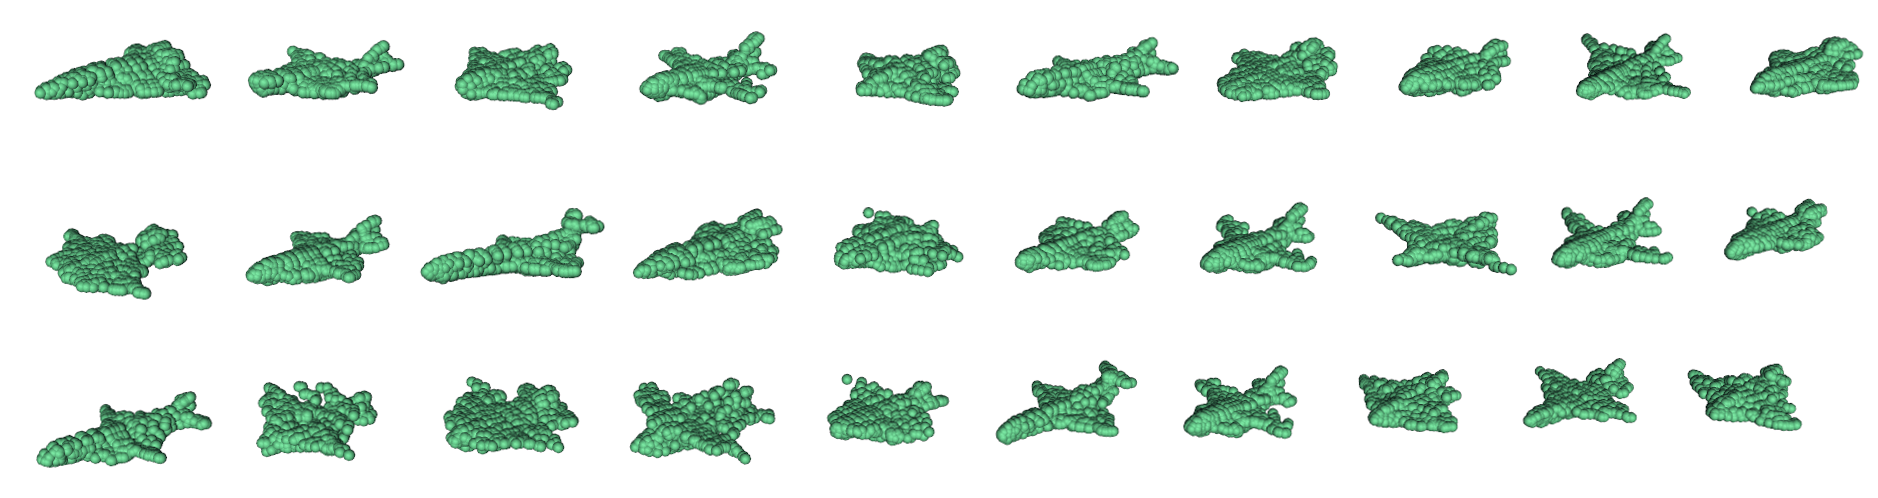
\includegraphics[width=1.0\linewidth]{PCAGAN/images/gallery/airplanes.png}

\includegraphics[width=1.0\linewidth]{PCAGAN/images/hline.png}
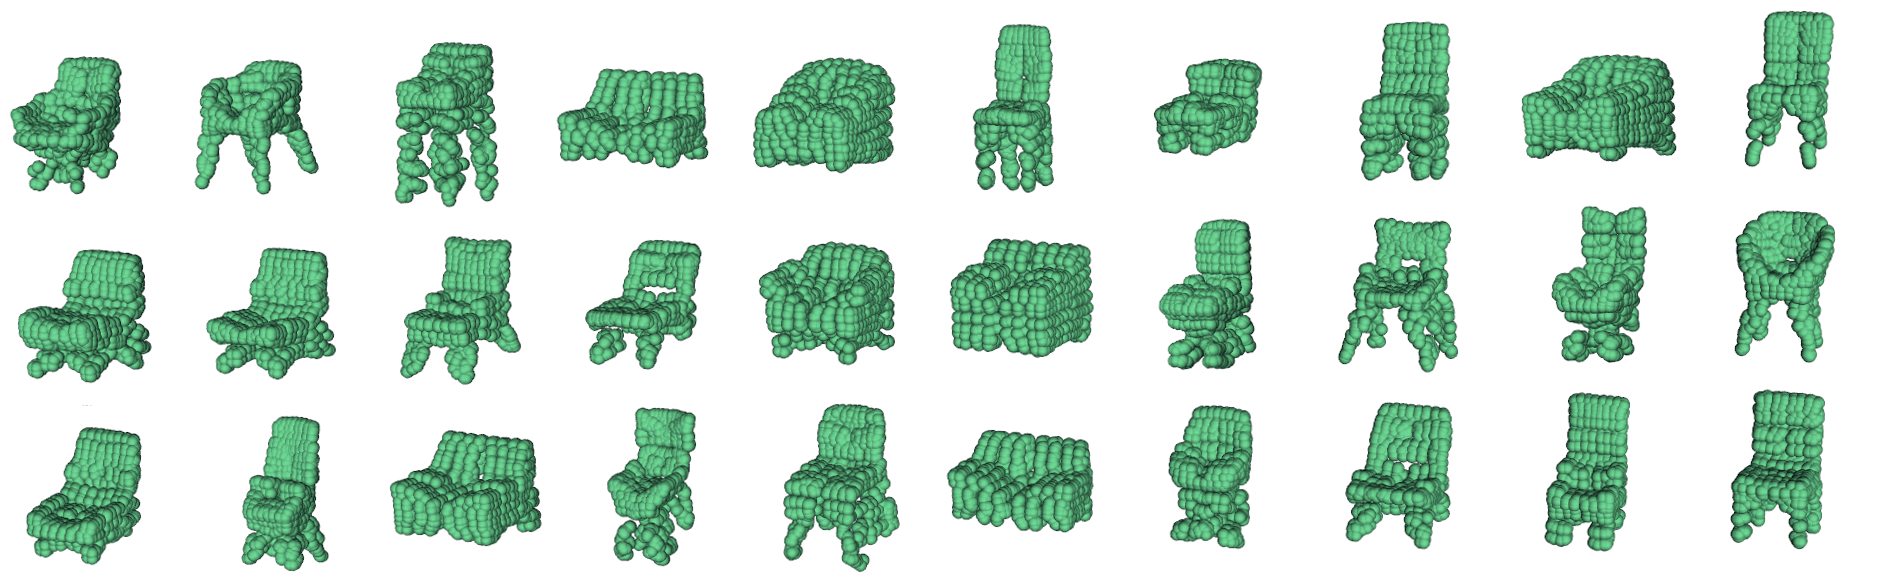
\includegraphics[width=1.0\linewidth]{PCAGAN/images/gallery/chairs.png}

\includegraphics[width=1.0\linewidth]{PCAGAN/images/hline.png}
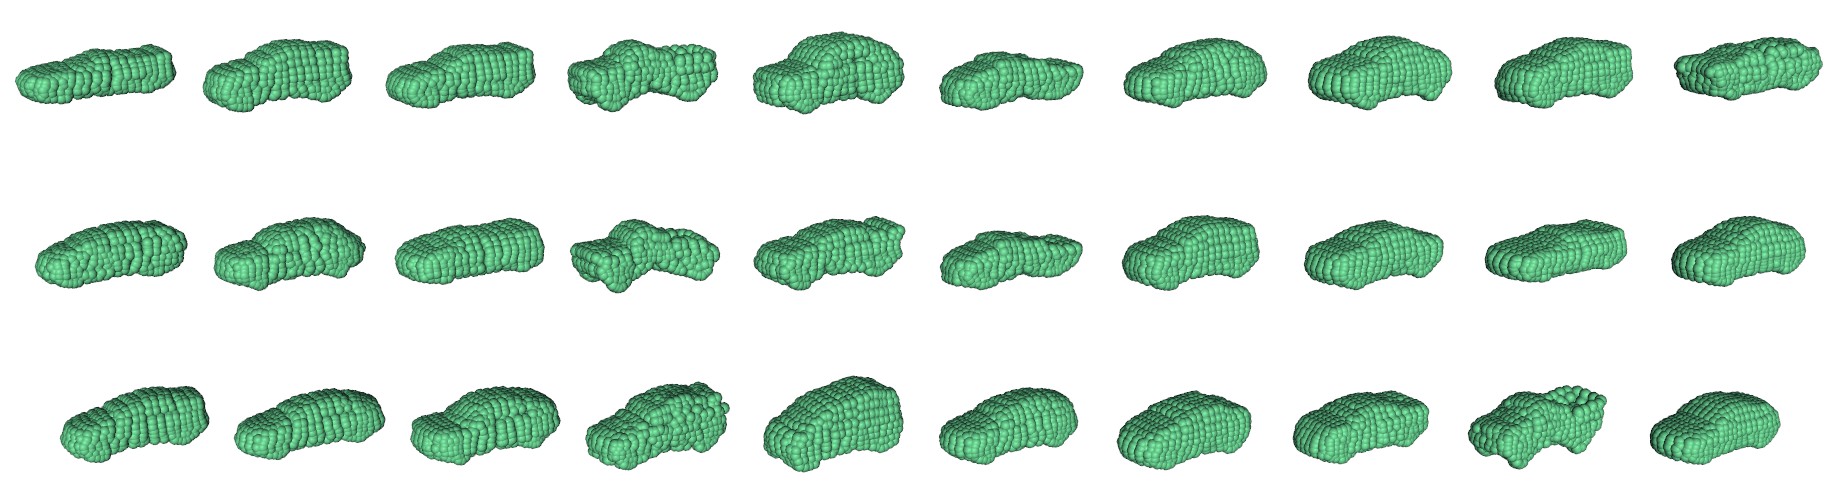
\includegraphics[width=1.0\linewidth]{PCAGAN/images/gallery/cars.png}
\vspace{-16pt}
\caption{\small \label{fig:gallery} A gallery showing results of using our method to generate points clouds for three categories: airplane, chair, and car. We use our method to train a GAN for each category separately. The training is generally very fast and completes within a few minutes. The results shown here are generated by randomly sampling the encoding $z$ of the GAN.}
\vspace{-12pt}
\end{figure}



